\chapter{Risultati del lavoro}
L'articolo originale presenta alcuni errori nell'illustrazione del metodo.\\
\section*{Correzione di una svista nell'articolo originale: inversione dei raporti di accettazione}
Nell'articolo \emph{Computational system identification for Bayesian
NARMAX modelling}  sul quale si è basata la mia implementazione si afferma che, per la mossa di morte riguardante il processo, la probabilità di accettazione è (secondo l'equazione 28)
\begin{equation}
\gamma_{death}^{(k)}=min\{1,r_a^{-1}\}
\end{equation}
l'affermazione si ripete analoga per il modello di rumore (equazione 34)
\begin{equation}
\gamma_{death}^{(q)}=min\{1,r_b^{-1}\}
\end{equation}
Dove si assume che $r_a$ e $r_b$ abbiano la stessa espressione dei rapporti di accettazione calcolati per le mosse di nascita (equazioni 35 e 29).\\
Queste formule sono errate, le formule giuste sono invece esattamente uguali a quelle per la mossa di nascita
\begin{equation}
\gamma_{death}^{(k)}=min\{1,r_a\}
\end{equation}
\begin{equation}
\gamma_{death}^{(q)}=min\{1,r_b\}
\end{equation}
senza effettuare il reciproco del rapporto.\\
La differenza tra il rapporto per le mosse di nascita e di morte è già contemplata nella diversa definizione di $k'$ nell'espressione del rapporto.\\
Il simbolo $k'$ infatti rappresenta il numero di termini proposto dalla mossa e vale rispettivamente $k+1$ per le mosse di nascita e $k-1$ per le mosse di morte.


\section*{Correzione di una svista nell'articolo originale: errore di segno in una formula}
Nell'articolo \emph{Computational system identification for Bayesian
NARMAX modelling} sul quale si è basata la mia implementazione, in particolare nell'equazione (42) è stato omesso un segno meno.
L'errore sembra essere sfuggito alla revisione.
La likehood corretta è infatti
\[p(y|P_k,E_q,a_k,b_q,\sigma_e^2)=\prod_{t=1}^N \exp \left(-\frac{\epsilon_t^2}{2\sigma_e^2}\right)\]
Questo errore è intuibile dato che il residuo è distribuito come una Gaussiana,
inoltre la likehood, nonostante sia scritta sotto forma di produttoria,dovrebbe essere la stessa dall'equazione (5) dove si legge il segno meno. In ogni caso per avvalorare la mia correzione ho  fatto un test sull'algoritmo in un caso banale. Questo test mi serve anche a validare il codice in un caso di studio estremamente semplificato .
\\
In questo caso il modello era fissato ad una costante scalare e venivano effettuate solo mosse di aggiornamento dei coefficienti.
Il vero modello era
\[y(t)=0.2+e(t)\]
con
\[\sigma_e= 0.07\]
Il modello con cui era stata inizializzata lidentificazione è
\[y(t)=0.4+e(t)\]
Ho graficato l'andamento del coefficiente identificato in funzione del numero di iterazioni
Di seguito l'andamento del coeffciente provando come dice l'articolo con il segno più.\\
\begin{figure}[ht]
\centering
\begin{minipage}[b]{0.45\linewidth}
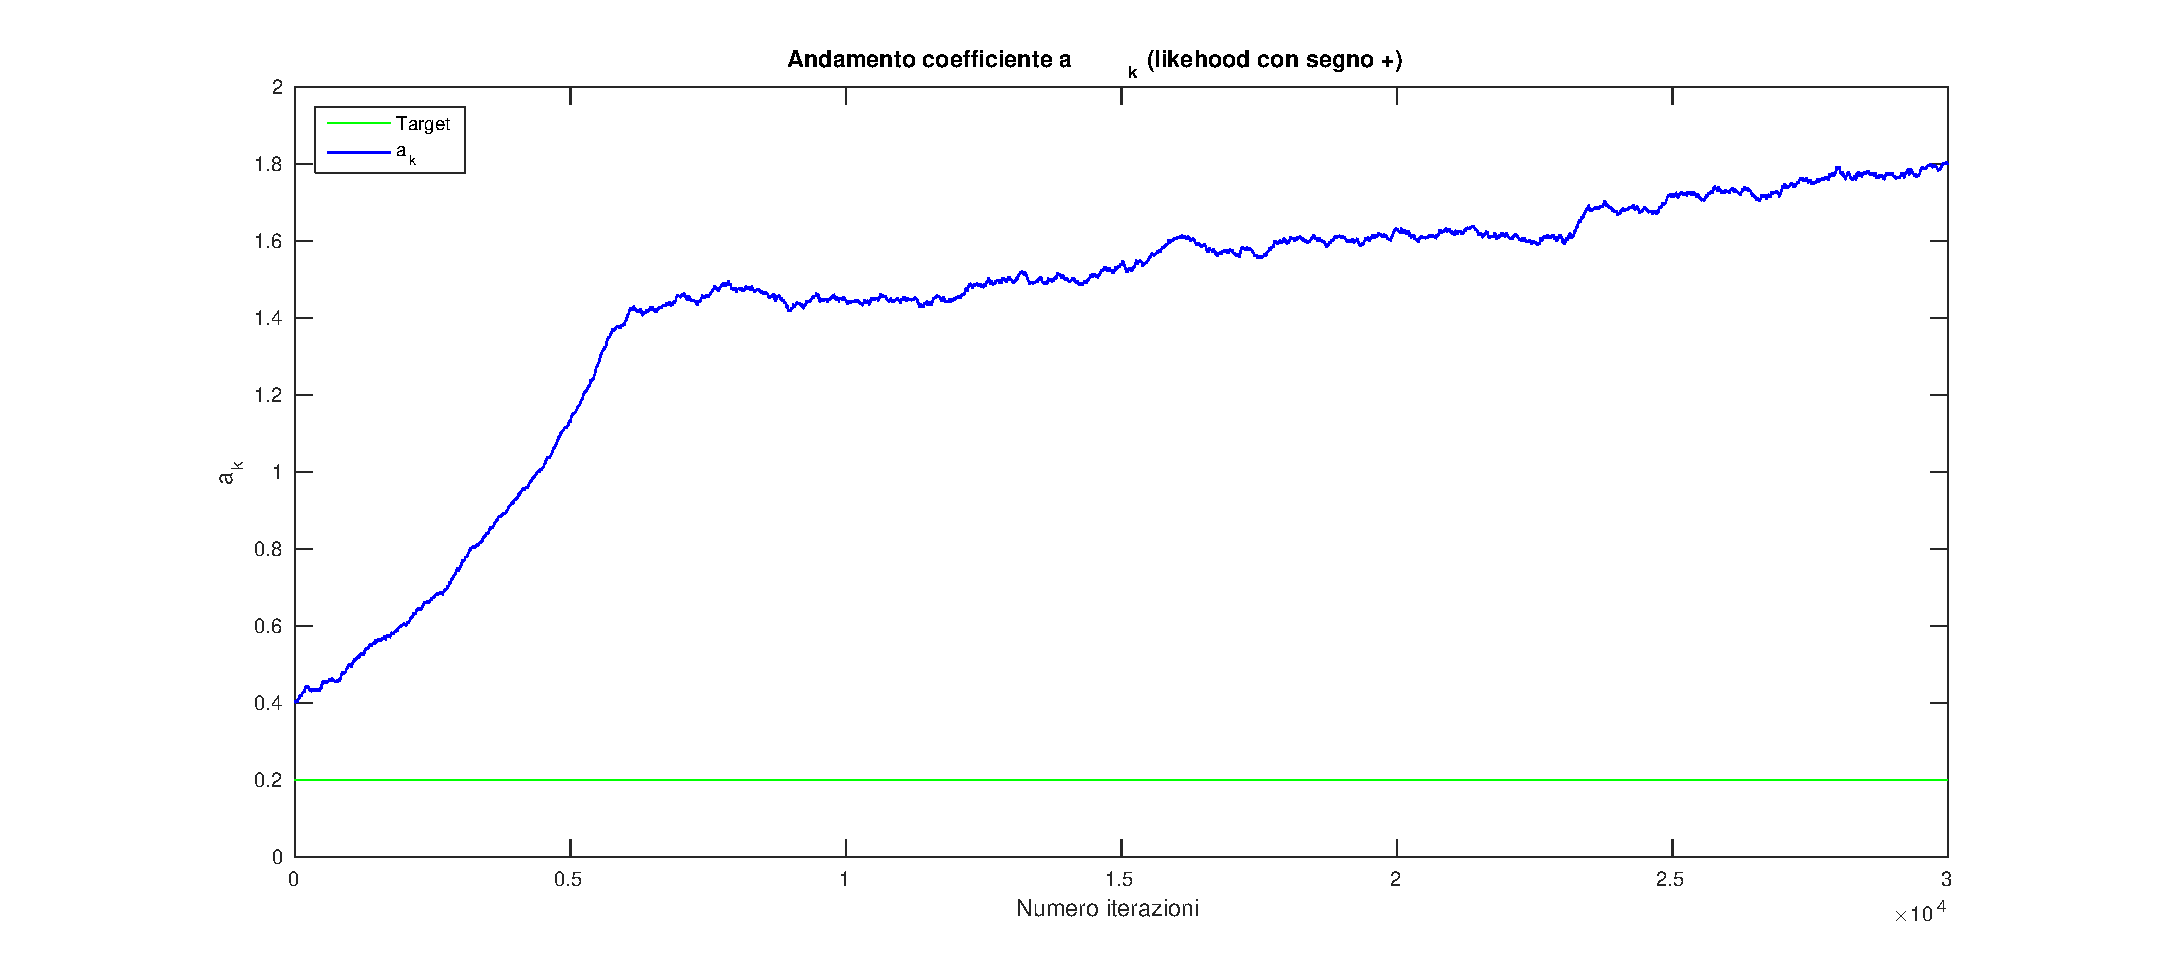
\includegraphics[scale=0.15]{akhplus.eps}
\caption{Serie temporale del coefficiente (segno più)}
\label{fig:minipage1}
\end{minipage}
\quad
\begin{minipage}[b]{0.45\linewidth}
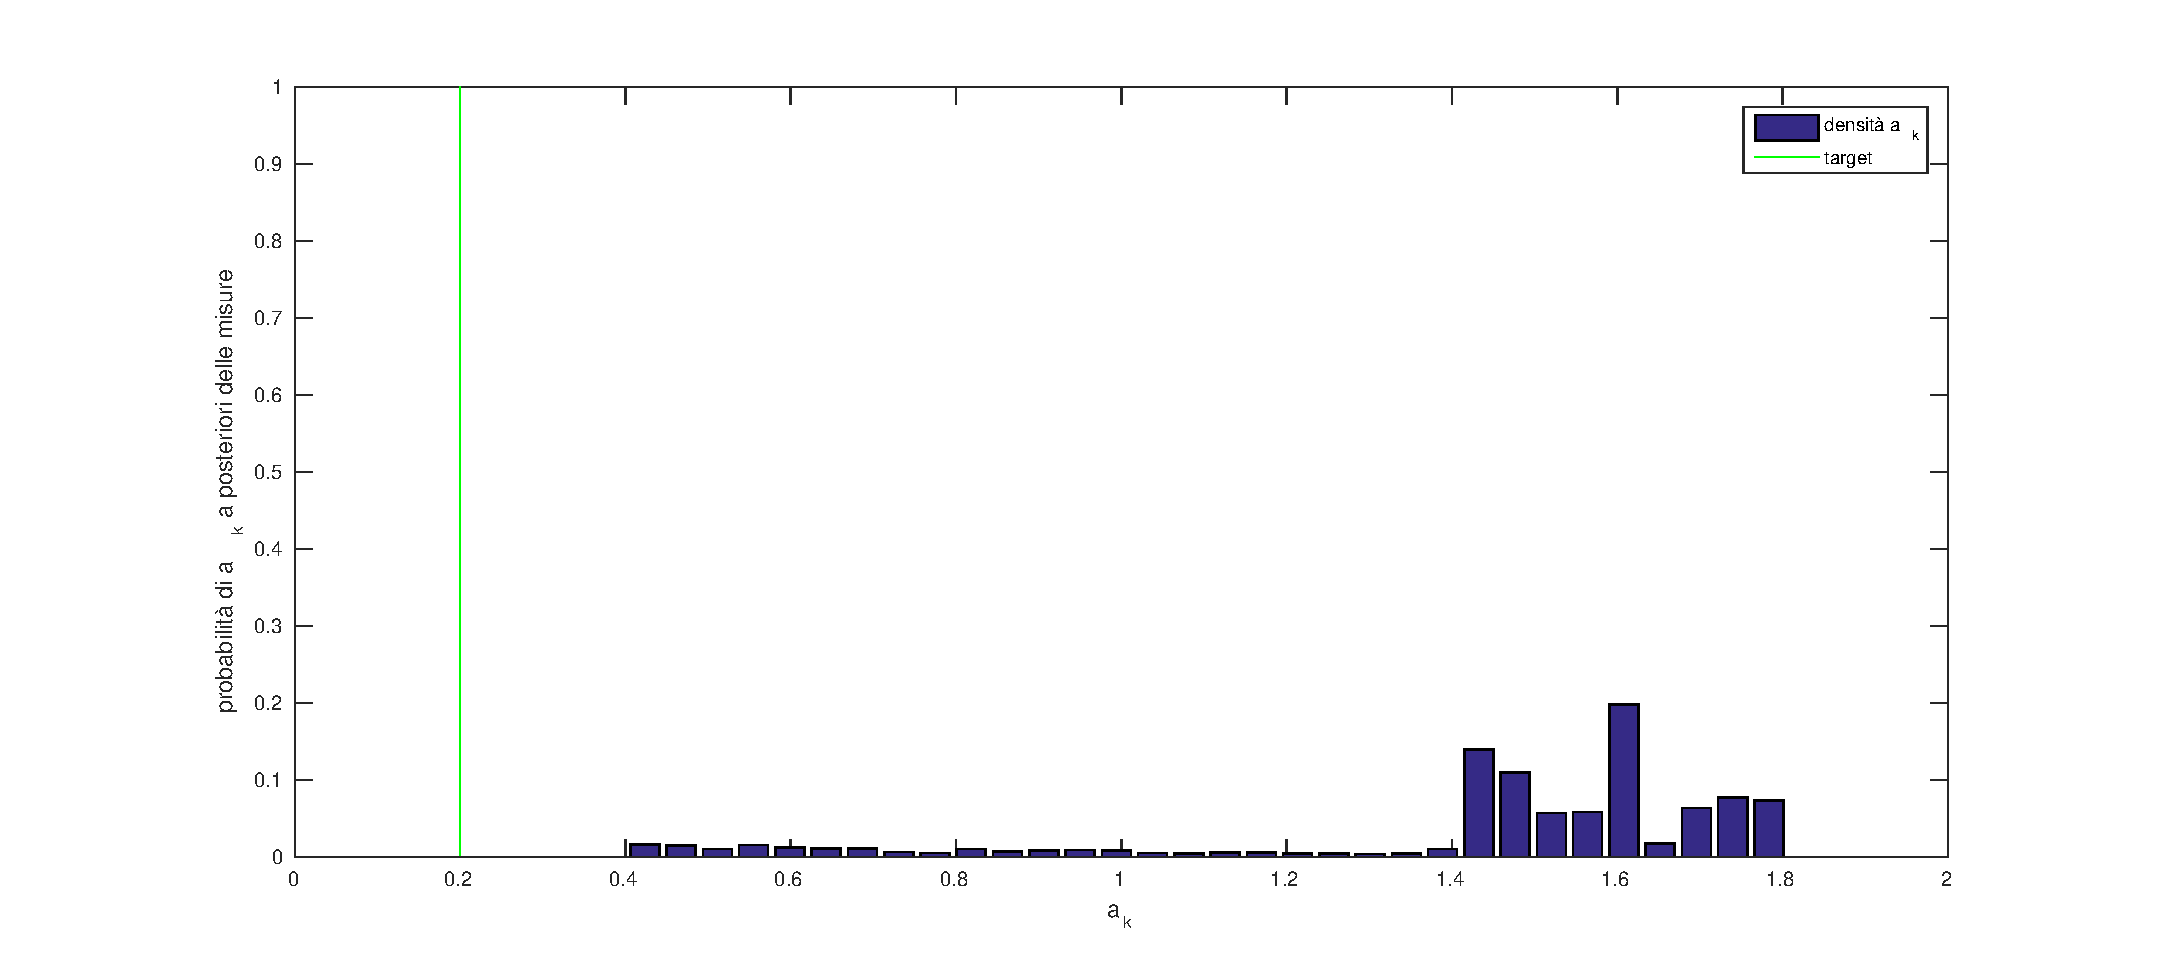
\includegraphics[scale=0.15]{p_ak_plus.eps}
\caption{Ddp a posteriori stimata del coefficiente (segno più)}
\label{fig:minipage2}
\end{minipage}
\end{figure}
\begin{figure}[ht]
\centering
\begin{minipage}[b]{0.45\linewidth}
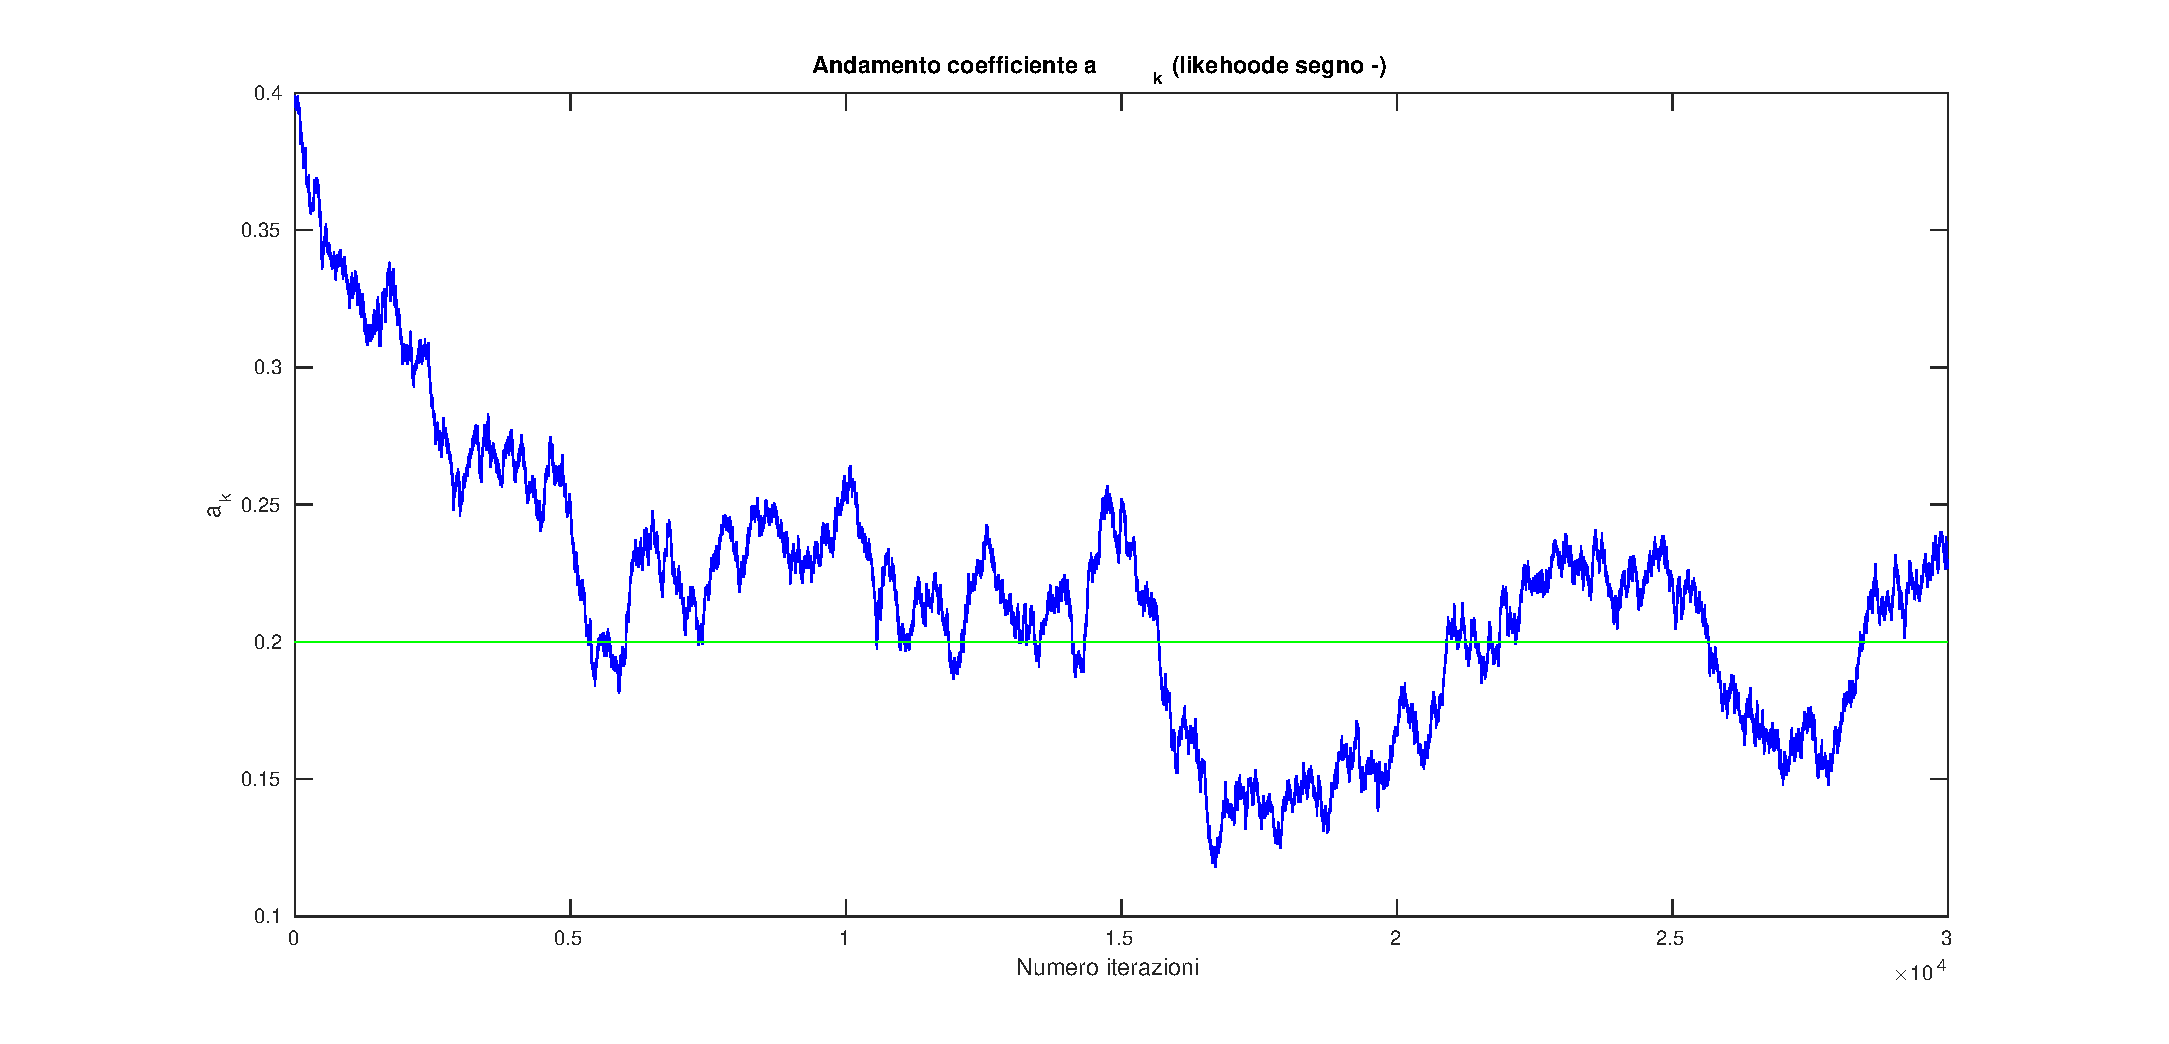
\includegraphics[scale=0.15]{akhminus.eps}
\caption{Serie temporale del coefficiente (segno meno)}
\label{fig:minipage1}
\end{minipage}
\quad
\begin{minipage}[b]{0.45\linewidth}
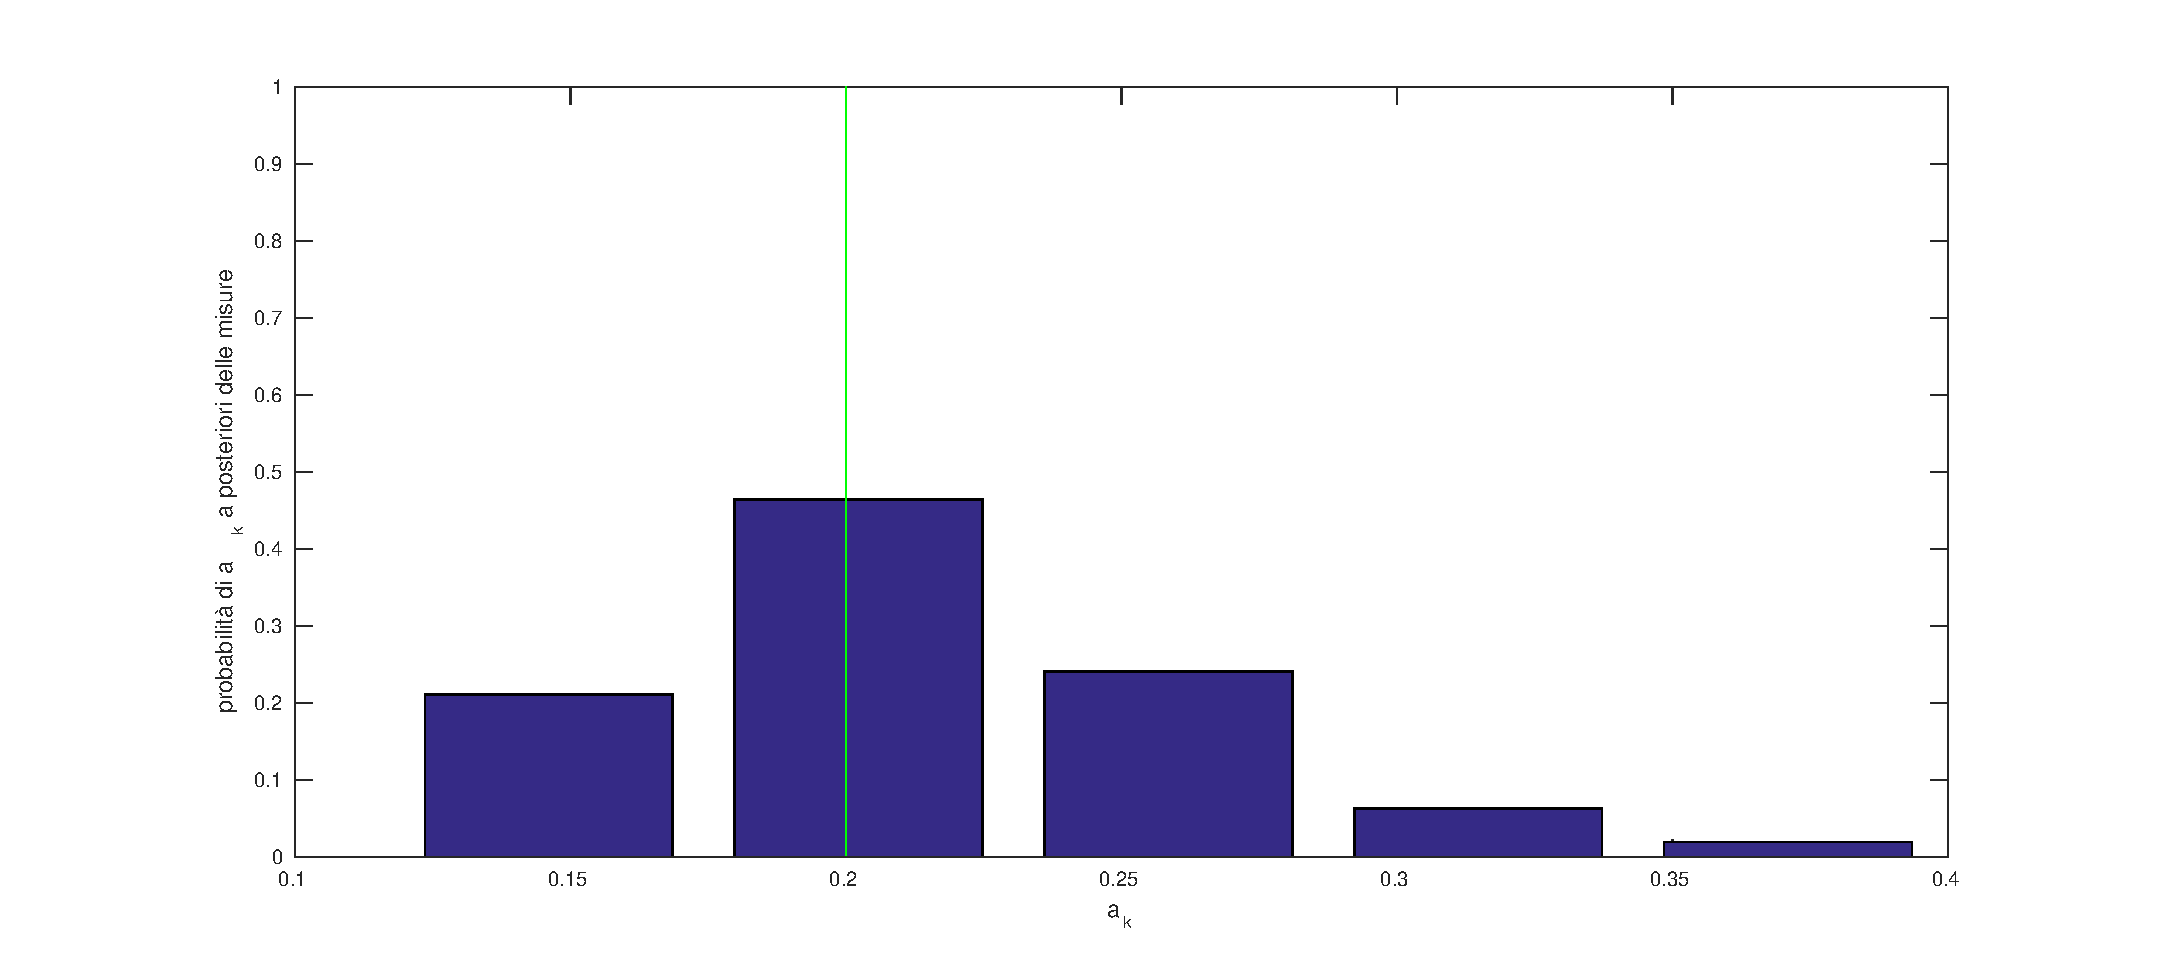
\includegraphics[scale=0.15]{p_ak_minus.eps}
\caption{Ddp a posteriori stimata del coefficiente (segno meno)}
\label{fig:minipage2}
\end{minipage}
\end{figure}

